\documentclass[conference]{IEEEtran}
\IEEEoverridecommandlockouts
% The preceding line is only needed to identify funding in the first footnote. If that is unneeded, please comment it out.
\usepackage{cite}
\usepackage{amsmath,amssymb,amsfonts}
\usepackage{algorithmic}
\usepackage{graphicx}
\usepackage{textcomp}
\usepackage{xcolor}
\usepackage[utf8]{inputenc}
\usepackage{float})
%\addbibresource{bibliografia.bib}
\def\BibTeX{{\rm B\kern-.05em{\sc i\kern-.025em b}\kern-.08em
    T\kern-.1667em\lower.7ex\hbox{E}\kern-.125emX}}
\begin{document}

\title{Trabalho 1 AC 3}

\author{\IEEEauthorblockN{1\textsuperscript{st} Rafael Augusto Barros Ladeira de Oliveira}
\IEEEauthorblockA{\textit{PUC Minas ICEI (Instituto de Ciências Exatas e Informática)} \\
\textit{Pontifical Catholic University of Minas Gerais (PUC Minas)}\\
Belo Horizonte, Minas Gerais, Brazil \\
rafael@theancientscroll.com}
\and
\IEEEauthorblockN{2\textsuperscript{nd} Henrique Mendonça Castelar Campos}
\IEEEauthorblockA{\textit{PUC Minas ICEI (Instituto de Ciências Exatas e Informática)} \\
\textit{Pontifical Catholic University of Minas Gerais (PUC Minas)}\\
Belo Horizonte, Minas Gerais, Brazil \\
henriquemendonacastelar@gmail.com}
}

\maketitle

\section{abstract}
The purpose of this article is to test the performance of a MIPS processor according to it’s specifications, which includes the size of the cache memory, the algorithm for replacing the data in the cache memory and the size of the cache line. For that, a program called Amnesia was used, a memory hierarchy simulator of a MIPS processor.\footnote{The program Amnesia can be download on this address: http://amnesia.lasdpc.icmc.usp.br/amnesia-en/}
%\Latex{abstract}

\begin{IEEEkeywords}
Amnesia, MIPS, Memory Hierarchy, Simulator, Replacement Algorithm, Computer Ar.
\end{IEEEkeywords}

\section{Introdução}
Um dos grande desafios da indústria dos microprocessadores é aumentar a performance de seus chips. Um dos fatores que interferem significativamente no desempenho de um microprocessador em um computador é a sua hierarquia de memória, que dependendo das configurações, pode aumentar ou diminuir o tempo necessário para acessar os dados que serão processados, o que poderá resultar em um alto ou baixo desempenho. Visando a entender um padrão que leve a um melhor desempenho, vários testes foram realizados no software Amnesia.

\section{Testes Realizados no Amensia}
O Amnesia é um projeto de Paulo Lopes e Sarita Bruschi, com a finalidade de ajudar alunos de engenharia da computação e derivados¸ a entender melhor hierarquia de memória de hardware computacional, para fins educacionais. Com ele estudantes e educadores simulam a atitude de diferentes registradores e processadores variando a memória cache, memoria virtual e paginada dos mesmos em diferentes cenários utilizando traces, instruções de acesso, leitura e .

Em cada teste realizado foi utilizada uma configuração diferente na máquina. Todos os testes rodaram o mesmo programa.

\subsection{Alteração dos Algoritmos de Substituição de Dados na Memoria Cache}

Durante os testes foi alternado entre os algoritmos de substituição de dados na memória cache. Os algoritmos utilizados foram o LRU (Least recently used) e o FIFO (First in first out). O LRU substitui o dado que foi menos recentemente utilizado, enquanto que o FIFO remove os dados na ordem em que eles foram inseridos.

\subsection{Alteração do Tamanho da Memória Cache}

Nos testes foram testado processadores com diferentes tamanhos de memória cache. O tamanho foi variado entre 8, 16 e 32 Bytes. Na teoria, quanto maior for o tamanho da memória cache menor será a taxa de não acertos (cache miss) o que resulta em um melhor desempenho. 

\subsection{Alteração do Tamanho da Linha da Memória Cache}

Nas configurações foram utilizados diferentes tamanhos de linha de memória cache. Os tamanhos variam entre 2, 4, 8 e 16 Bytes.

\subsection{Funcionamento do Amnesia}

\begin{figure}[H]
  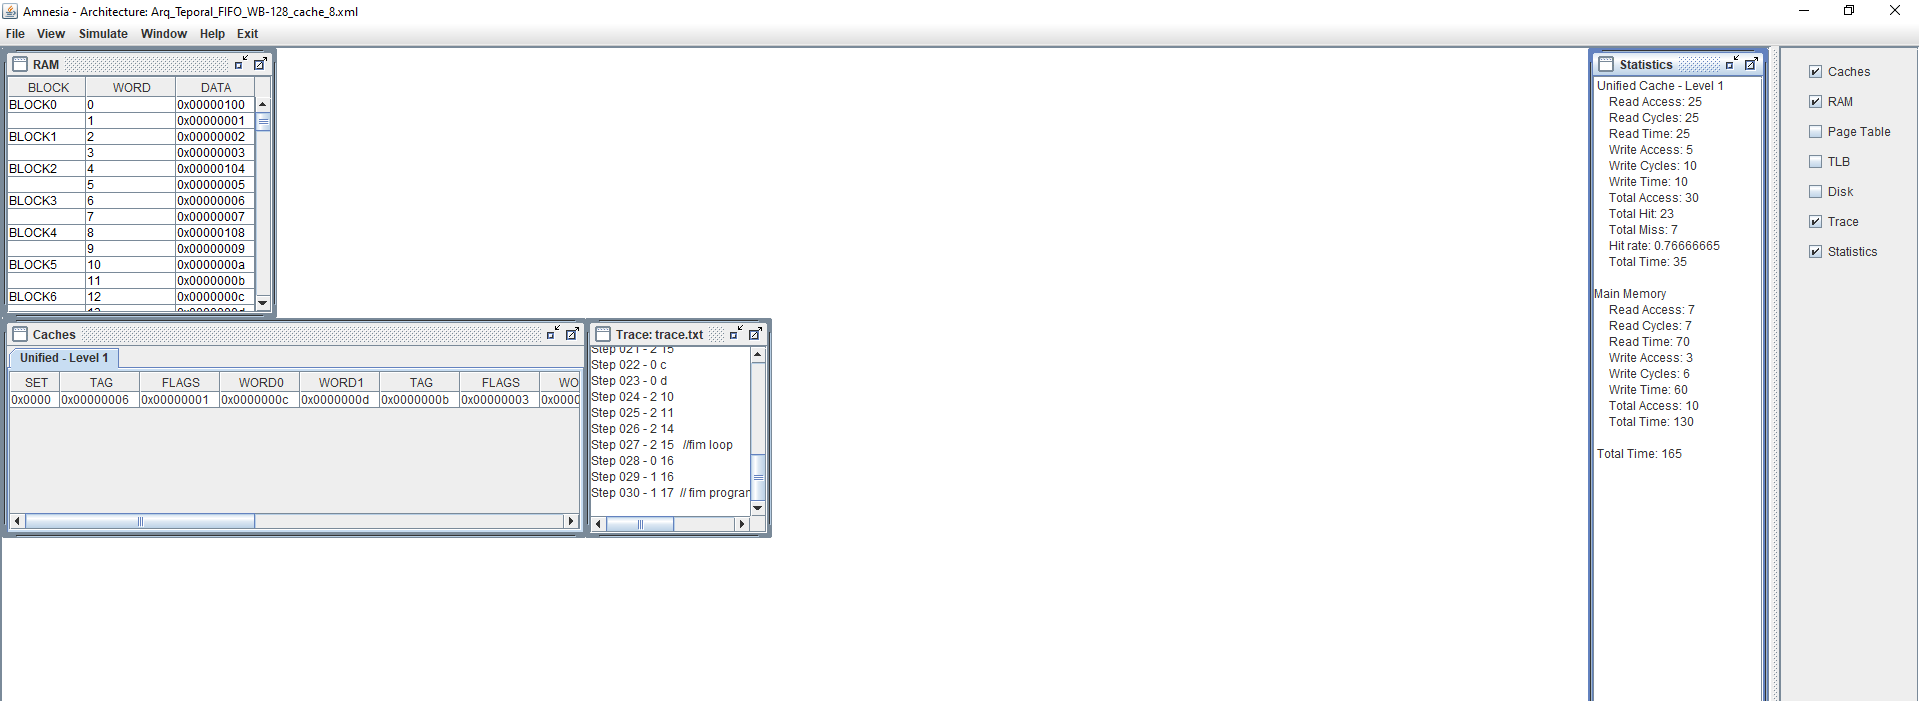
\includegraphics[width=\linewidth]{Amnesia_screen.png}
  \caption{Tela do Programa Amnesia fazendo um teste}
  \label{fig:Tela do Programa Amnesia fazendo um teste}
\end{figure}

\begin{itemize}
\item  
Geral . \\
O simulador nos permite gerar diferentes cenários de simulações de leitura e escrita de dados
customizando as configurações de hierarquia de mémoria a partir da alteração de diversas configurações da memoria. Exemplo FIFO ou LRU e seu memory size, cache size e line size dentre outros. Além disso podemos testar diversos cenáriso diferentes para uma mesma memória e como ela se comportaria para os varios cenários criados para testar suas capacidades, quando incluimos os mesmos no programa apartir dos seus arquivos traces. Logo, uma simulação nunca tera os mesmos resultados.\\
\\

\item Arquivo de Configuração de Arquitetura. \\
A base da simulação, os arquivos formatados em xml são onde todas as configuração do processador e sua hierarquia de memoria. Nele customizamos a memoria cache, principal e virtual, line size, block size dentre outras configurações. È baseado nesses dados que o desempenho ao executar ações do trace variam de configuração para configuração.
\\

\item Traces. \\
\begin{figure}[H]
  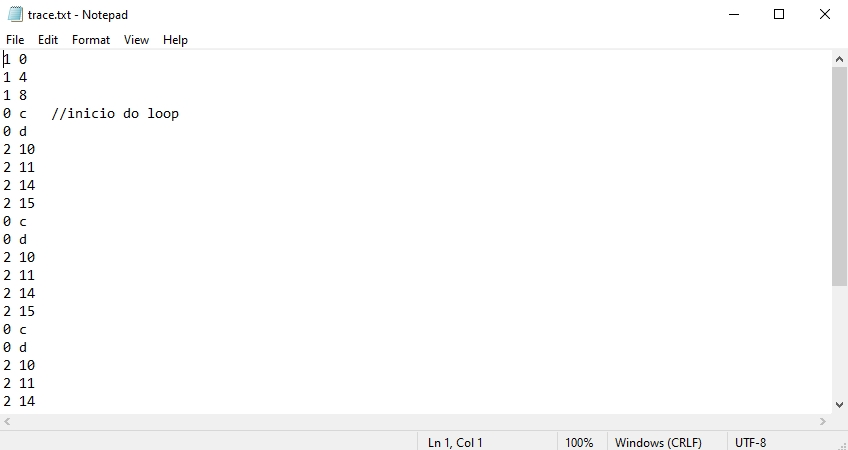
\includegraphics[width=\linewidth]{trace.jpg}
  \caption{Arquivo trace com várias instruções de leitura, escrita, busca de instrução e registro escape}
  \label{fig:trace}
\end{figure}
Os arquivos traces são  arquivos normalmente na extensão txt contendo as instruções de acesso que serão realizadas pela nossa arquitetura de memoria da simulação no prograama Amnesia. Neles as ações são divididas em 5 tipos de instruções. Onde as de rótulo 0 executam a leitura de dados, 1 gravação de dados, 2 busca de instrução, 3 registro escape(tratado como tipo de acesso desconhecido) e por ultímo a 4 que é registro escape(operação cache de flush)
Apartir dos chamados traces criamos instruções para testar as capacidades dos processadores. Onde o 
\
\\
\item Arquitetura em Arquivos XML. \\

\begin{figure}[H]
  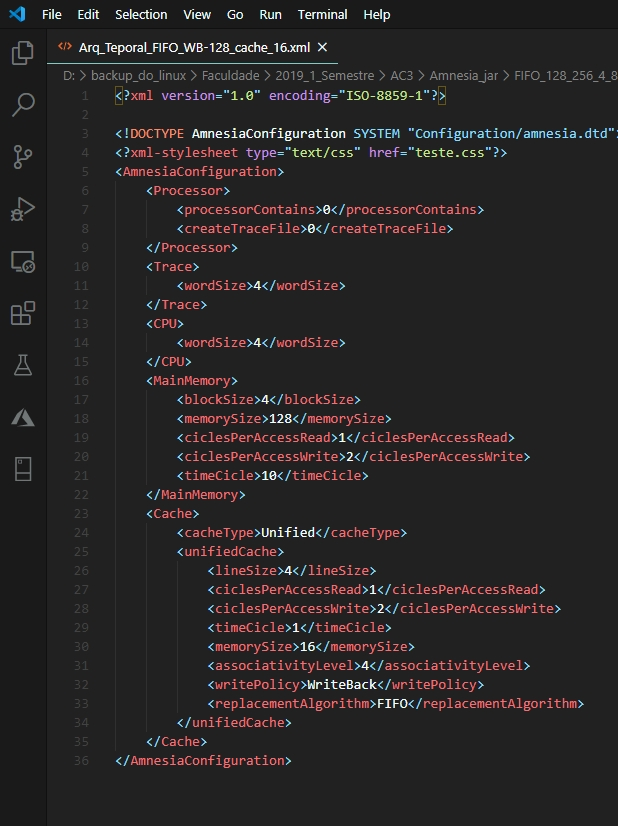
\includegraphics[width=\linewidth]{arquitetura_de_memoria.jpg}
  \caption{Exemplo de um arquivo contendo um processador, configurações da memoria principal e virtual dentre outras configurações para ser testado na simulação do amnesia}
  \label{fig:Tela do Programa Amnesia fazendo um teste}
\end{figure}

Os arquivos traces são  arquivos normalmente na extensão txt contendo as instruções de acesso que serão realizadas pela nossa arquitetura de memoria da simulação no programa Amnesia. Neles as ações são divididas em 5 tipos de instruções. Onde as de rótulo 0 executam a leitura de dados, 1 gravação de dados, 2 busca de instrução, 3 registro escape(tratado como tipo de acesso desconhecido) e por ultimo a 4 que é registro escape(operação cache de flush)
Apartir dos chamados traces criamos instruções para testar as capacidades dos processadores.
\

\end{itemize}

\section{Arquiteturas Utilizadas}
 Para executarmos nossos testes utilizaremos das arquiteturas LRU (Least Recently Used Page) e a FIFO(First-in First-out).
\\
\begin{itemize}
\item LRU (Least Recently Used Page)
O Algoritmo de memória (Least Recently Used) tem como objetivo organizar as páginas a partir das que tiverem maior chance de serem bastante utilizadas nas novamente. Na troca a página que permaneceu em desuso pelo maior tempo.  O maior problema dele é seu alto custo, pois deve-se manter lista encadeada com todas as páginas que estão na memória, com as mais recentes utilizadas no início e as menos utilizadas no final; Essa lista deve ser atualizada a cada referência da memória,
\\
\item FIFO (First-in First-out)
\\
O Algoritmo de memória( First-in First-out) Page Replacement, ele trabalha mantendo uma fila das páginas correntes na memória. Onde a página no início da fila é a mais antiga e a página no final é a mais nova. Porém quando ocorre um page fault a atual página do início é remove e a nova é inserida ao final da fila. Ele é considerado por muitos simples, entretando podendo ser ineficiente em alguns casos, como quando uma pagina que está em uso constante tende a ser retirada.

\end{itemize}
\\
\section{Resultados dos Testes}

\begin{figure}[H]
%    \centering
    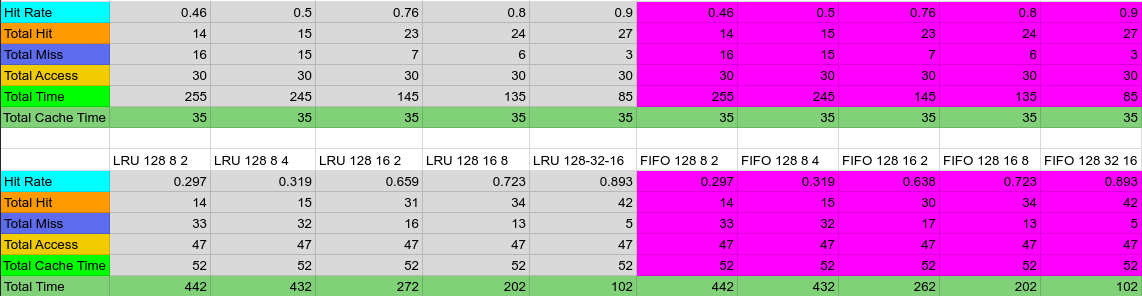
\includegraphics[width=\linewidth]{Imagens/Tabela.png}
    \caption{Comparação das taxas de acerto entre FIFO e LRU.\break Na tabela de cima a memória virtual está desabilitada. Já na tabela de baixo a memória virtual está habilitada}
    \label{fig:Comparação das taxas de acerto entre FIFO e LRU. Na tabela de cima a memória virtual está desabilitada. Já na tabela de baixo a memória virtual está habilitada}
\end{figure}

Na comparação da taxa de acertos na memória cache não houve diferença significativa entre a política de substituição FIFO e LRU, como mostra a figura 5.

\begin{figure}[H]
%    \centering
    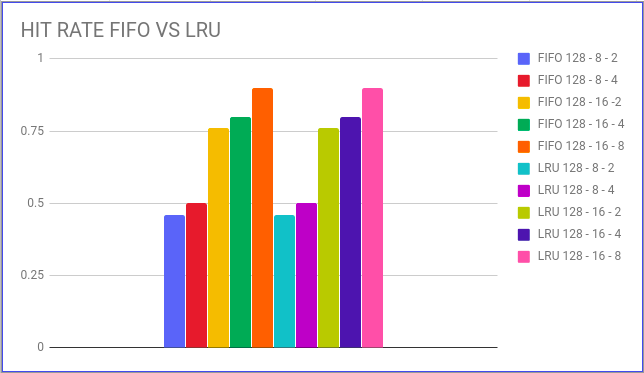
\includegraphics[width=\linewidth]{Imagens/Hit_RATE_FIFO_VS_LRU.png}
    \caption{Taxa de acerto na memória cache em FIFO vs LRU}
    \label{fig:Taxa de acerto na memória cache em FIFO vs LRU}
\end{figure}


Além disso, os testes mostram que quanto maior for a taxa de acerto (na maioria das vezes), maior será o tempo de escrita, como mostra na figura 6. Porém há pontos do gráfico que isso não necessariamente ocorre.

\begin{figure}[H]
%    \centering
    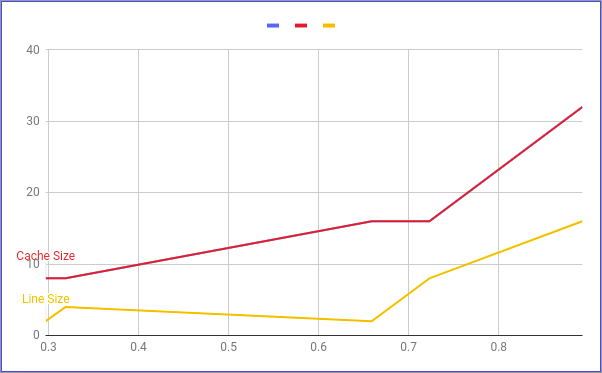
\includegraphics[width=\linewidth]{Imagens/WRITE_TIME_POR_HIT_RATE.png}
    \caption{Tempo de escrita por taxa de acerto na memória cache}
    \label{fig:Tempo de escrita por taxa de acerto na memória cache}
\end{figure}

Ademais, foi comprovado (como esperado na teoria) que quanto maior for a memória cache maior será a taxa de acertos na memória cache, como mostra nos gráficos 5 e 7.

\begin{figure}[H]
%    \centering
    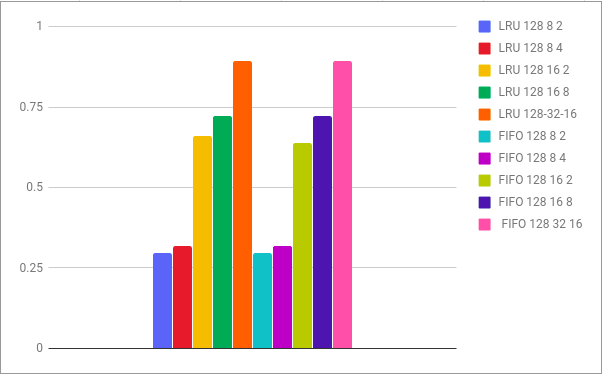
\includegraphics[width=\linewidth]{Imagens/HIT_RATE_POR_ARQUITETURA.png}
    \caption{Taxa de acerto por arquitetura}
    \label{fig:Taxa de acerto por arquitetura}
\end{figure}



\section{Conclusão}

Durante a realização deste trabalho, muito foi aprendido sobre a hierarquia de memória, tamanho da memória cache, tamanho do bloco, e o algoritmo de substituição e como essas configurações interferem na performance do microprocessador. 

\section{Referências Bibliográficas}

\begin{thebibliography}{9}
\bibitem{latexcompanion} 
Michel Goossens, Frank Mittelbach, and Alexander Samarin. 
\textit{The \LaTeX\ Companion}. 
Addison-Wesley, Reading, Massachusetts, 1993.

\bibitem{einstein} 
Albert Einstein. 
\textit{Zur Elektrodynamik bewegter K{\"o}rper}. (German) 
[\textit{On the electrodynamics of moving bodies}]. 
Annalen der Physik, 322(10):891–921, 1905.

\bibitem{knuthwebsite} 
Knuth: Computers and Typesetting,
\\\texttt{http://www-cs-faculty.stanford.edu/\~{}uno/abcde.html}
\end{thebibliography}


\end{document}
